\documentclass[degree=bachelor, tocarialchapter]{bnuthesis}
% 选项
%   degree=[bachelor|master|doctor|postdoctor], % 必选,学位类型
%   secret,                % 可选(默认:关闭),是否有密级
%   tocarialchapter,       % 可选(默认:关闭),章目录中使用黑体(这项表示同时打开下面两项)
%   tocarialchapterentry,  % 可选(默认:关闭),单独控制章标题在目录中使用黑体
%   tocarialchapterpage,   % 可选(默认:关闭),单独控制章页码在目录中使用黑体
%   pifootnote,            % 可选(默认:关闭),页脚编号采用 pifont 字体符号,建议打开

% 所有其它可能用到的包都统一放到这里了,可以根据自己的实际添加或者删除。
\usepackage{bnuthesis}

% 定义所有的图片文件在 figures 子目录下
\graphicspath{{figures/}}

% 可以在这里修改配置文件中的定义。导言区可以使用中文。
% \def\myname{薛瑞尼}

\begin{document}

%%% 封面部分
\frontmatter
\bnusetup{
  %******************************
  % 注意:
  %   1. 配置里面不要出现空行
  %   2. 不需要的配置信息可以删除
  %******************************
  %
  %=====
  % 中文信息
  %=========
  ctitle={ 等温捷径与绝热捷径构成的类卡诺热机的功率与效率},
  cdegree={理学学士},
  cdepartment={物理学系},
  cmajor={物理学},
  cauthor={龚政楠},
  csupervisor={涂展春教授},
  cassosupervisor={涂展春教授}, % 校内
  % 日期自动使用当前时间,若需指定按如下方式修改:
  %=========
  % 英文信息
  %=========
  etitle={Finite Time Thermodynamics},
  edegree={Bacholar of Science},
  emajor={Physics},
  eauthor={R.Z},
  esupervisor={XXX},
  eassosupervisor={XXXX},
  % 日期自动生成,若需指定按如下方式修改:
  % edate={December, 2005}
  %
  % 关键词用“英文逗号”分割
  ckeywords={有限时间热力学, 等温捷径, 绝热捷径, 类卡洛热机},
  ekeywords={TeX, LaTeX, CJK, template, thesis}
}

% 定义中英文摘要和关键字
\begin{cabstract}
  论文的摘要是对论文研究内容和成果的高度概括。摘要应对论文所研究的问题及其研究目
  的进行描述,对研究方法和过程进行简单介绍,对研究成果和所得结论进行概括。摘要应
  具有独立性和自明性,其内容应包含与论文全文同等量的主要信息。使读者即使不阅读全
  文,通过摘要就能了解论文的总体内容和主要成果。

  论文摘要的书写应力求精确、简明。切忌写成对论文书写内容进行提要的形式,尤其要避
  免“第 1 章……;第 2 章……;……”这种或类似的陈述方式。

  本文介绍清华大学论文模板 \bnuthesis{} 的使用方法。本模板符合学校的本科、硕士、
  博士论文格式要求。

  本文的创新点主要有:
  \begin{itemize}
    \item 用例子来解释模板的使用方法;
    \item 用废话来填充无关紧要的部分;
    \item 一边学习摸索一边编写新代码。
  \end{itemize}

  关键词是为了文献标引工作、用以表示全文主要内容信息的单词或术语。关键词不超过 5
  个,每个关键词中间用分号分隔。(模板作者注:关键词分隔符不用考虑,模板会自动处
  理。英文关键词同理。)
\end{cabstract}

% 如果习惯关键字跟在摘要文字后面,可以用直接命令来设置,如下:
% \ckeywords{\TeX, \LaTeX, CJK, 模板, 论文}

\begin{eabstract}
   An abstract of a dissertation is a summary and extraction of research work
   and contributions. Included in an abstract should be description of research
   topic and research objective, brief introduction to methodology and research
   process, and summarization of conclusion and contributions of the
   research. An abstract should be characterized by independence and clarity and
   carry identical information with the dissertation. It should be such that the
   general idea and major contributions of the dissertation are conveyed without
   reading the dissertation.

   An abstract should be concise and to the point. It is a misunderstanding to
   make an abstract an outline of the dissertation and words ``the first
   chapter'', ``the second chapter'' and the like should be avoided in the
   abstract.

   Key words are terms used in a dissertation for indexing, reflecting core
   information of the dissertation. An abstract may contain a maximum of 5 key
   words, with semi-colons used in between to separate one another.
\end{eabstract}

% \ekeywords{\TeX, \LaTeX, CJK, template, thesis}
% 如果使用授权说明扫描页,将可选参数中指定为扫描得到的 PDF 文件名,例如:
% \makecover[scan-auth.pdf]
\makecover
 
%% 目录
\tableofcontents

%% 符号对照表
\begin{denotation}[3cm]
  \item[$E$] 能量
  \item[$m$] 质量
  \item[$c$] 光速
  \item[$P$] 概率
  \item[$h$] 普朗克常量,$6.62607015 \times 10^{-34}\  \M{J \cdot s}$
  \item[$\hbar$] 约化普朗克常量,$\hbar \equiv \frac{h}{2\pi}$
  \item[$\PP{f}{\bm{r}}$] 定义为$\sum \PP{f}{r_i} \hat{r}_i$ 

\end{denotation}



%%% 正文部分
\mainmatter
\chapter{引言:热机的最大功率与效率问题}
热机的发明和使用对人类的生产生活产生了重大的影响,第一次工业革命和第二次工业革命都和热机的发展有紧密的关系. 一直以来,特别是近些年来,由于能源短缺的问题愈发突出,研究热机的效率问题吸引着一大批研究者.

早在1824,卡诺就指出(基于热质说)\cite{2005}:工作在相同高温热源和相同低温热源的所有热机中,以可逆热机的效率最高,而且这些可逆热机的效率都相同. 为$\eta _{\text{C}}=1-\frac{T_1}{T_2}$ 。这个问题似乎就这么解决了,然而必须注意的是可逆热机的要求相当于要求工作物质是准静态的. 也就是说,要想严格意义上达到卡诺热机的效率,热机一个循环的工作时间应当是无限长,这样的热机功率是0.

我们当然不可能接受功率为0的热机,所以得到热机保持在某一功率下(特别是最大功率)的最大效率成了摆在我们面前的问题,而这个问题促进了有限时间热力学的诞生. 

1975年,Curzon和Ahlborn研究了内可逆热机\cite{Curzon1975},该热机可在有限时间内完成一个循环. 利用Newton热运输规律,得到了该热机在最大功率下的效率为$\eta _{CA}=1-\sqrt{T_c/T_h}=1-\sqrt{1-\eta _C}$ ,其中$\eta _\text{C}$为卡诺效率。

2008年,T. Schmiedl 和 U. Seifert提出了布朗随机热机模型\cite{Schmiedl2008},该热机模型利用谐振子势场驱动布朗粒子做功,并得到了其在最大功率下的效率 . 

同年,涂展春推导出费曼棘轮热机\cite{Tu2008}在最大功率下的效率$\eta _{\text{F}}=\frac{\eta _{\text{C}}^{2}}{\eta _{\text{C}}-\left( 1-\eta _{\text{C}} \right) \ln \left( 1-\eta _{\text{C}} \right)}$. \cite{Tu2020}

……

同时涂展春\cite{Tu2008}在小温差条件下,即$\eta _{\text{C}}\rightarrow 0$. 将上述热机的效率按照 展开. 发现这些效率到二阶项都相同的,它们都普遍地满足$\eta _{\text{U}}=\frac{\eta _{\text{C}}}{2}+\frac{\eta _{\text{C}}^{2}}{8}+O\left( \eta _{\text{C}}^{3} \right)$. 这个规律在其他热机中也得到了验证,但也有一些热机不满足这个关系. 这引发了研究者对相关问题的思考,涂展春在紧耦合热机的范畴内对其中的原因进行了解释.\cite{Tu2020}

在这些形形色色的有限时间热机中,由Seifert等人提出的随机热机\cite{Schmiedl2008}占据一席之地. 随机热机通常是利用外势驱动与热源接触的布朗粒子做功. 其中的具体的实现过程可以有很大的不同,对应着不同的随机热机. 在这些不同的随机热机中, Campo等人利用绝热捷径构建的奥托热机\cite{DelCampo2014}引人注目. 而后,Deng等人发现绝热捷径能够提高奥托热机的效率,不论是经典的还是量子的.\cite{Deng2013} 涂展春在Schmiedl和Seifert工作\cite{Schmiedl2008}的基础上,考虑了他们在过阻尼情况下忽略的惯性的影响,构建了一种类卡洛热机\cite{Tu2013}. 惊讶地发现这种随机热机的效率等于Curzon和Ahlborn构建的内可逆热机\cite{Curzon1975}的效率 . 在涂展春构建的热机中\cite{Tu2013},布朗粒子在与时间相关的谐振子$U=\lambda ^2\left( t \right) x^2/2$的控制下,经历了类卡诺循环. 其中与卡诺循环中绝热过程对应的就是前面提到的绝热捷径,但与卡诺循环中等温过程对应的“等温过程”,却只是粒子与恒温热源接触,而非系统保持等温. 

这促使笔者思考是否有与卡诺循环中等温过程更加对应的过程,以实现类卡诺循环. 等温捷径\cite{Li2016}的提出为实现这个目标提供了契机,李耿等人给一个系统引入了辅助势,这个系统的演化本来是被一个含时哈密顿量所决定的,这个精心选择的辅助势可以使得系统在当前的哈密顿量下的状态,仿佛处于原哈密顿量的瞬时平衡态中一样,从而实现了“等温过程”,我们称之为等温捷径.

综上,笔者欲构造由绝热捷径和等温捷径构成的类卡诺循环,根据随机热力学和非平衡热力学中的典型方法,研究该热机工作过程中的功、熵、能量损失等参数,并考察它的效率与功率. 并与其他类型的热机,特别是涂展春构建的类卡洛热机\cite{Tu2013}进行比较,Campo等人构建的奥托热机\cite{DelCampo2014}. 考虑到Deng等人发现绝热捷径能够提高奥托热机的效率\cite{Deng2013},我们也期望等温捷径的引入能进一步提高热机的效率



\section{背景介绍:热机的功率与效率}
封面的例子请参看 \texttt{cover.tex}。主要符号表参看 \texttt{denation.tex},附录和
个人简历分别参看 \texttt{appendix01.tex} 和 \texttt{resume.tex}。里面的命令都很直
观,一看即会\footnote{你说还是看不懂?怎么会呢?}。

\section{字体命令}


\chapter{随机热机}
\section{随机热力学}

\section{随机热机模型}

\section{绝热捷径}
\qquad 在有限时间热力学中,一个非常重要的议题是如何实现不同平衡态的相互转换。因为\textbf{有限时间}的限制使得我们不能够使用准静态的方法,而绝热捷径\cite{Chen2010}提供了这样一种可以在有限时间内实现平衡态转化的策略。这个策略是由 Demirplak and Rice \cite{Demirplak2003}和 Berry \cite{Berry2009} 独立发展出来的。\R{(两篇文章相隔太久,很奇怪,出自\cite{Jarzynski2013})}在这个策略发展处以后的很长一段时间内,它引起了一大批研究者的关注。下面我们回顾一下绝热捷径是怎么实现的。

考虑量子力学中的绝热定理\cite{Griffiths2018}:如果一个系统的哈密顿量$H_0(t)$随时间变化很缓慢,即$\tau_\mathrm{e} \gg \tau_\mathrm{i}$,其中$\tau_\mathrm{e}, \tau_\mathrm{i}$分别表示环境的特征时间和系统的内部特征时间。那么如果系统在时间$t=0$处于$H_0 (0)$的本征态,即系统的初态$| \psi(0) \rangle = | n(0) \rangle$,绝热定理告诉我们系统在$t$时刻会处于$H_0 (t)$的对应于瞬时本征态$| n(0) \rangle$,并且
\begin{equation}
    |\psi(t)\rangle=|n(t)\rangle e^{i \theta_{n}(t)} e^{i \gamma_{n}(t)}
    \label{eq2.1}
\end{equation}

其中$\theta_{n}(t)=-\frac{1}{\hbar} \int_{0}^{t} E_{n}(t^{\prime}) \M{d} t^{\prime}, \gamma_{n}(t)=i \int_{0}^{t}\langle n(t^{\prime}) | \partial_{t^{\prime}}n(t^{\prime})\rangle \M{d} t^{\prime}$

不难注意到,绝热定理实现了$H_0(t)$的对应的本征态之间的转化$| n(0) \rangle \to | n(t) \rangle$。现在我们考虑取消$\tau_\mathrm{e} \gg \tau_\mathrm{i}$的要求。

假设存在一个哈密顿量$H(t)$,它使得系统的态的演化严格为$|\psi(t)\rangle=|n(t)\rangle e^{i \theta_{n}(t)} e^{i \gamma_{n}(t)}$,则根据薛定谔方程有
\begin{equation}
    i \hbar \PP{t} |\psi(t)\rangle= H(t) |\psi(t)\rangle
    \label{eq2.2}
\end{equation}

将\ref{eq2.1}代入\ref{eq2.2},整理得$ E_{n}+ i \hbar \left( | \partial_{t} n \rangle -\langle n | \partial_t n \rangle\right)|n\rangle=H| n\rangle$,于是可得
\begin{align}
    \nonumber H(t)&=H_{0}(t)+i \hbar \sum_{m}\left(\left|\partial_{t} m\right\rangle\left\langle m\left|-\left\langle m \mid \partial_{t} m\right\rangle\right| m\right\rangle\langle m|\right) \\
    &\equiv H_0 + H_1
    \label{eq2.3} 
\end{align}

于是一个以$H (t)$作为哈密顿量的系统,若其初态为$H_0 (t)$的本征态$| n(0) \rangle$,那么不论$H (t)$随时间的变化快慢与否,在$t$时刻,系统的状态依然是$H_0 (t)$的本征态,只是两者有一个相位差。于是我们实现了在有限时间内的本征态之间的转化。这其中的关键在于我们引进了一个\textbf{反绝热哈密顿量}$H_1 (t)$,根据\ref{eq2.3},我们已经在形式上得到了$H_1 (t)$。现在我们考虑对于具体的$H_0 (t)$,如何得到$H_1 (t)$的具体表达式。\cite{Jarzynski2013}

让$H_0$通过一系列参数$\bm{\lambda}(t)=\left( \lambda_1 (t) , \lambda_1 (t) , \lambda_1 (t) , \cdot , \lambda_{N} (t) \right)$依赖于时间$t$。同时,$H_0 (\bm{\lambda})$的本征值、本征态为$E_n (\bm{\lambda}), | n (\bm{\lambda}) \rangle$,根据复合函数的微分法则,式\ref{eq2.4}可以写为
\begin{equation}
    H_1 (t)=\dot{\boldsymbol{\lambda}} \cdot \boldsymbol{\xi}(\boldsymbol{\lambda}(t))
    \label{eq2.5}
\end{equation}
其中
\begin{equation}
    \boldsymbol{\xi}(\boldsymbol{\lambda})=i \hbar \sum_{m}(|\boldsymbol{\nabla} m\rangle\langle m|-\langle m \mid \boldsymbol{\nabla} m\rangle| m\rangle\langle m|)
    \label{eq2.4}
\end{equation}
同时$|\nabla m\rangle \equiv \partial_{\boldsymbol{\lambda}}|m(\boldsymbol{\lambda})\rangle  , \dot{\boldsymbol{\lambda}} \equiv \mathrm{d} \lambda / \mathrm{d} t$

把$\boldsymbol{\xi}$看做参数空间的无穷小平移$\boldsymbol{\lambda} \to \boldsymbol{\lambda} + \delta \boldsymbol{\lambda}$的生成元。这个无穷小平移与希尔伯特空间中态的变换$|\psi\rangle \rightarrow|\psi\rangle+|\delta \psi\rangle$相联系,通过以下方式
\begin{equation}
    i \hbar|\delta \psi\rangle=\delta \boldsymbol{\lambda} \cdot \boldsymbol{\xi}|\psi\rangle
    \label{eq2.6}
\end{equation}
这样,在一阶近似下,$H_0 (\bm{\lambda})$的本征态$|n(\bm{\lambda})\rangle$的变换为\R{(有一点不懂,额外的相位怎么出来的\cite{Jarzynski2013})}
\begin{equation}
    |n(\boldsymbol{\lambda})\rangle \rightarrow\left(1+\frac{1}{i \hbar} \delta \boldsymbol{\lambda} \cdot \hat{\boldsymbol{\xi}}\right)|n(\boldsymbol{\lambda})\rangle=e^{i \delta \boldsymbol{\lambda} \cdot \boldsymbol{A}_{n}}|n(\boldsymbol{\lambda}+\delta \boldsymbol{\lambda})\rangle
    \label{eq2.7}
\end{equation}
其中$\boldsymbol{A}_{n}(\boldsymbol{\lambda})=i\langle n | \boldsymbol{\nabla} n\rangle.$ 这意味着,沿着参数空间的曲线$\bm{\lambda}$利用式\ref{eq2.7},可以将系统的态逐步从$|n(\M{\lambda_0})\rangle$变换成$\M{e}^{i \int_{\bm{\lambda_0}}^{\bm{\lambda_s}}   i\langle n | \boldsymbol{\nabla} n\rangle \M{d}\bm{\lambda}}\left|n\left(\boldsymbol{\lambda}_{s}\right)\right\rangle.$ 这正是们所希望得到的形式。

现在看看系统态的时间演化,先考虑系统经过一个无穷小时间$\delta t$,则态$|\psi \rangle$将演化为
\begin{equation}
     \left(1+\frac{1}{i \hbar} H \delta t\right)|\psi\rangle=|\psi\rangle+\frac{1}{i \hbar} \delta t H_{0}|\psi\rangle+\frac{1}{i \hbar} \delta \boldsymbol{\lambda} \cdot \boldsymbol{\xi}|\psi\rangle
   \label{eq2.8}
\end{equation}

如果考虑态$|\psi \rangle = |n(\bm{\lambda}) \rangle$,那么\ref{eq2.8}的物理意义是明显的。$H_0$产生了我们熟悉的动力学相位,而$\boldsymbol{\xi}$产生了几何相因子。

由\ref{eq2.4}定义的$\bm{\xi}$,也可由下式\ref{eq2.9}定义,(二者的等价性可由$\langle m \mid \boldsymbol{\nabla} n\rangle=\left\langle m\left|\boldsymbol{\nabla} \hat{H}_{0}\right| n\right\rangle /\left(E_{n}-E_{m}\right)$\cite{Berry2009}加以证明)
\begin{subequations}
    \begin{align}
        \left[ \boldsymbol{\xi}, H_{0} \right] &= i \hbar \left( \boldsymbol{\nabla} H_{0}-\operatorname{diag} \left(\boldsymbol{\nabla} H_{0} \right) \right) \label{eq2.9a}\\
        \langle n|\boldsymbol{\xi}| n\rangle &= 0 \label{eq2.9b}
    \end{align}
    \label{eq2.9}
\end{subequations}
其中$\operatorname{diag}\left(\boldsymbol{\nabla} H_{0}\right)=\sum_{m}|m\rangle\left\langle m\left|\boldsymbol{\nabla} H_{0}\right| m\right\rangle\langle m|.$ 对\ref{eq2.9a}两端同时进行操作$\langle m|\cdots| n\rangle$,得到$\langle m| \boldsymbol{\xi} | n\rangle (E_n - E_m) = \langle m|i \hbar \left( \boldsymbol{\nabla} H_{0}-\operatorname{diag} \left(\boldsymbol{\nabla} H_{0} \right) \right)| n\rangle$. 可见,\ref{eq2.9a}决定了$\boldsymbol{\xi}$的非对角元,\ref{eq2.9b}决定了其非对角元。

式\ref{eq2.9}提供了一种在经典力学中找到\textbf{反绝热哈密顿量}的对应方法。因为我可以利用量子与经典的对应$[A, B]/i \hbar \to \{A, B\}  $将\ref{eq2.9}转换为经典的,进而可以在经典力学中找到对应的\textbf{反绝热哈密顿量}。现在考虑一个经典系统,其自由度为1,哈密顿量为$H_0 (\bm{\eta};\bm{\lambda}).$ 其中$\bm{\lambda}$依然为依赖于时间的一系列参数,$\bm{\eta}=(q,p)$为广义坐标和广义动量,确定了相空间的一个点。对于确定的能量$E = H_0 (\bm{\eta};\bm{\lambda})$,这将相点约束在相空间的一个能壳上,积分
\begin{equation}
    I(E, \boldsymbol{\lambda}) \equiv \int \mathrm{d} \bm{\eta} \theta\left[E-H_{0}(z ; \boldsymbol{\lambda})\right]
  \label{eq2.10}
\end{equation}
表示的是能壳所围成的体积,阶跃函数$\theta\left[E-H_{0}(z ; \boldsymbol{\lambda})\right]$可以使得积分区域为整个相空间。经典的绝热定理告诉我们$I(E, \boldsymbol{\lambda})$是一个\textbf{绝热不变量}\cite{LiuChuan2019}。也就是说如果$H_0$随时间$t$变化的足够缓慢,那么能壳所围成的体积将保持不变。定义任意可观测量$A$的\textbf{微正则分布平均}
\begin{equation}
    \langle A \rangle_{E, \lambda} \equiv \frac{1}{\partial_{E} I} \int \mathrm{d} \bm{\eta} \delta\left(E-H_{0}\right) A
  \label{eq2.11}
\end{equation}
利用函数$I (E,\bm{\lambda})$去定义函数$E (I, \bm{\lambda})$,则有
\begin{equation}
    \boldsymbol{\nabla} E(I, \boldsymbol{\lambda})=-\frac{\boldsymbol{\nabla} I(E, \boldsymbol{\lambda})}{\partial_{E} I(E, \boldsymbol{\lambda})}=\left\langle\boldsymbol{\nabla} H_{0}\right\rangle_{E, \boldsymbol{\lambda}}
  \label{eq2.12}
\end{equation}
其中第一个等式利用循环函数的偏导数的性质,第二个等式利用了式\ref{eq2.10}和式\ref{eq2.11}。

式\ref{eq2.9}的经典对应为\cite{Jarzynski1995}
\begin{subequations}
    \begin{align}
        \left\{\boldsymbol{\xi}, H_{0}\right\} &=\boldsymbol{\nabla} H_{0}-\left\langle\boldsymbol{\nabla} H_{0}\right\rangle_{E, \boldsymbol{\lambda}} \equiv \boldsymbol{\nabla} \tilde{H}_{0}    \label{eq2.13a}\\
        \langle\boldsymbol{\xi}\rangle_{E, \boldsymbol{\lambda}} &=0 \label{eq2.13b}
    \end{align}
    \label{eq2.13}
\end{subequations}
其中$\{ \cdots \}$是经典力学中的泊松括号$\{A, B\}=(\partial A / \partial q)(\partial B / \partial p)-(\partial A / \partial p)(\partial B / \partial q)$。利用式\ref{eq2.12}和泊松括号的定义,式\ref{eq2.13a}可改写为\R{不懂,出自\cite{Jarzynski2013} page2 (13)}
\begin{equation}
    \{\boldsymbol{\xi}, i\}=\boldsymbol{\nabla} i
  \label{eq2.14}
\end{equation}
其中关于$\bm{\eta}$和$\bm{\lambda}$的函数$i$的定义为:$i (\bm{\eta}; \bm{\lambda}) \equiv I \left( H_0\left( \bm{\eta}; \bm{\lambda}\right) ; \bm{\lambda} \right)$。类似于量子的情形的,将$\boldsymbol{\xi} (\bm{\eta}; \bm{\lambda})$看做和参数空间的无穷小平移$\boldsymbol{\lambda} \to \boldsymbol{\lambda} + \delta \boldsymbol{\lambda}$相联系的相空间的平移$\bm{\eta} \to \bm{\eta} + \delta \bm{\eta}$的生成元,有\cite{H.1986}
\begin{equation}
    \delta \bm{\eta}=\delta \boldsymbol{\lambda} \cdot\{\bm{\eta}, \boldsymbol{\xi}\}
  \label{eq2.15}
\end{equation}
于是,由式\ref{eq2.14}和\ref{eq2.15}可得
\begin{align}
    &i(\bm{\eta}+\delta \bm{\eta} ; \boldsymbol{\lambda}+\delta \boldsymbol{\lambda})-i(\bm{\eta} ; \boldsymbol{\lambda}) \\
    =&\frac{\partial i}{\partial \bm{\eta}} \delta \bm{\eta}+\boldsymbol{\nabla} i \cdot \delta \boldsymbol{\lambda} \\
    =&(\{i, \boldsymbol{\xi}\}+\nabla i) \cdot \delta \boldsymbol{\lambda}=0
    \label{eq2.16}
\end{align}
这说明,变换$\bm{\eta} \to \bm{\eta} + \delta  \bm{\lambda} \cdot \{\bm{\eta}, \boldsymbol{\xi}\}$将能壳$H_{0}(\bm{\eta} ; \boldsymbol{\lambda})$上的一个相点映射到能壳$H_{0}(\bm{\eta} + \delta \bm{\eta} ; \boldsymbol{\lambda})$上的一个点,而二者包围着相同的相体积。

可见,类似于量子中的情形,只要给经典的系统施加一个反绝热的哈密顿量$\dot{\boldsymbol{\lambda}} \cdot \boldsymbol{\xi}(\bm{\eta}, \boldsymbol{\lambda}(t))$。那么此系统的$I(E, \boldsymbol{\lambda}) \equiv \int \mathrm{d} \bm{\eta} \theta\left[E-H_{0}(z ; \boldsymbol{\lambda})\right]$将严格保持不变,不论$H_0 $随时间的变化快慢与否。这个新的哈密顿量为\R{(文献\cite{Jarzynski2013} page eq16直接计算了$\DD{}{t} i (\bm{\eta}; \bm{\lambda})$,但其中的推理过程未能理解)}
\begin{equation}
    H(\bm{\eta}, t)=H_{0}(\bm{\eta} ; \boldsymbol{\lambda}(t))+\dot{\boldsymbol{\lambda}} \cdot \boldsymbol{\xi}(\bm{\eta}, \boldsymbol{\lambda}(t))
    \label{eq2.17}
\end{equation}

\emph{从系综的角度来考虑这个过程:想象一下从H0的能壳E0中取样的初始条件的集合。在任何后来的时间t>0,从这些初始条件演化出来的轨迹,在Hamiltonian H(z; t)下,将填充一个H0(z;(t))的单一能壳E(t),具体来说是绝热能壳,它与初始能壳的相空间体积相同。如果我们把绝热能壳想象成一个随着参数随时间变化而变形的闭合循环,那么在式16中,H0围绕这个循环产生运动,调整每个轨迹,使其保持在壳上。}\R{可不要,出自\cite{Jarzynski2013} page eq16}

现在,鉴于变换$\bm{\eta} \to \bm{\eta} + \delta  \bm{\lambda} \cdot \{\bm{\eta}, \boldsymbol{\xi}\}$将能壳$H_{0}(\bm{\eta} ; \boldsymbol{\lambda})$ 上的相点映射到了能壳 $ H_{0}(\bm{\eta} + \delta \bm{\eta} ; \boldsymbol{\lambda})$上,我们可以此为根据构造经典力学中的$\boldsymbol{\xi}(\bm{\eta}, \boldsymbol{\lambda})$,下面我们用例子进行说明

\begin{itemize}
    \item 一维盒子中的粒子
\end{itemize}
考虑一个一维的粒子,处在两堵刚性墙之间,刚性墙的位置为$q=0,L$,这个例子这对应于量子力学中的一维无限深势阱。其相空间的能壳如图\ref{p2.1}所示。
\begin{figure}[!htbp]
    \begin{center}
        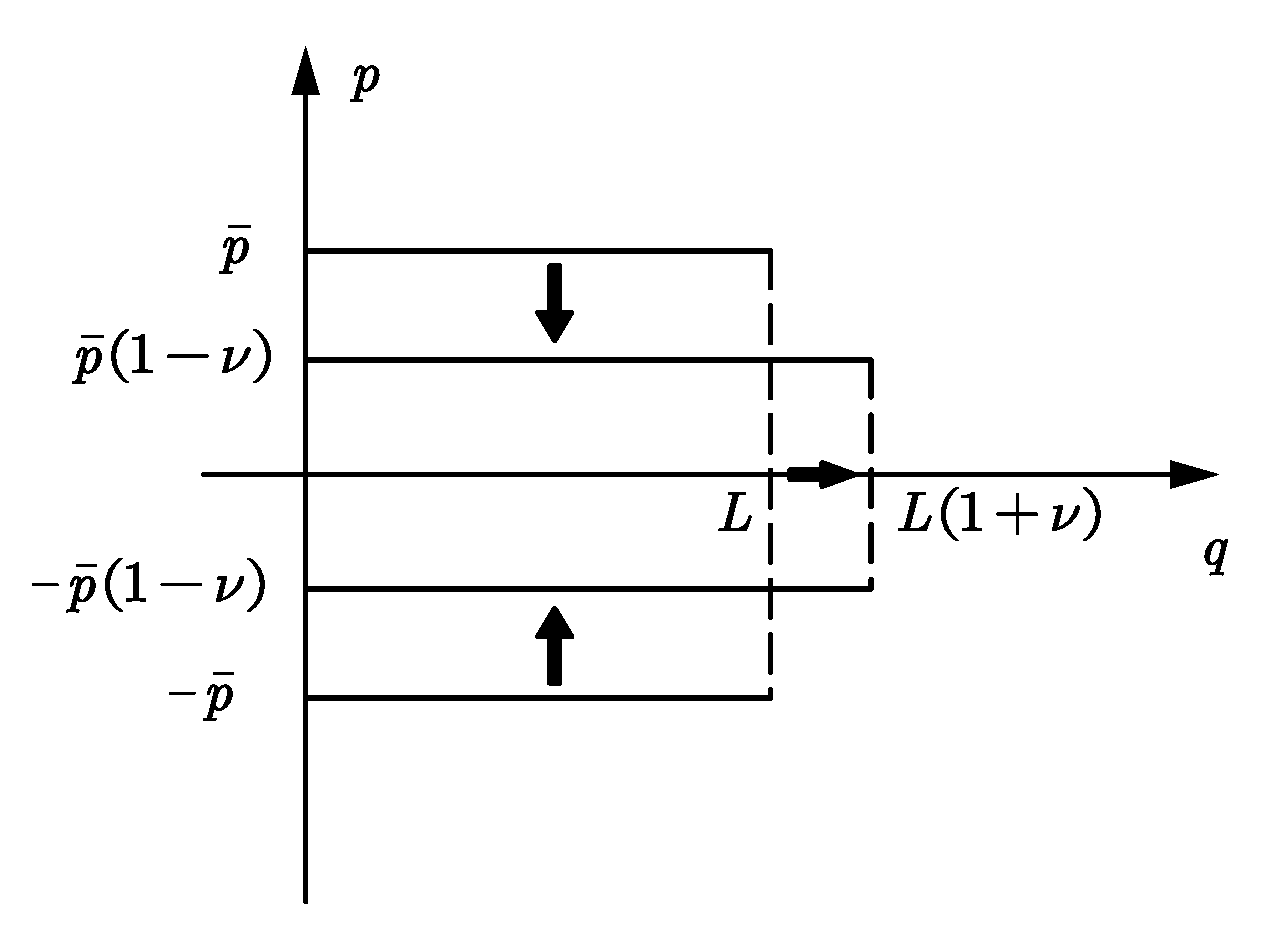
\includegraphics[width=0.5\textwidth]{figures/p2.1.pdf}
    \end{center}
    \caption{在一维盒子中的粒子的能壳。该粒子的能壳是一个矩形,当盒子的长度发生极小的改变时,矩形能壳也发生相应的改变。但矩形的体积不变}
    \label{p2.1}
\end{figure}

系统的哈密顿量为
\begin{equation}
     H_{0}(\bm{\eta} ; L)=\frac{p^{2}}{2 m}+V_{\mathrm{box}}(q ; L)
        \label{eq2.18}
\end{equation}
其中$V_{\mathrm{box}}(q ; L)$代表一维盒子的势场$V_{\mathrm{box}}(q ; L) = \left\{\begin{array}{l} 0 ,\ q<L\\ \infty ,\ q \leq 0\ or\ q \geq L \end{array}\right.$在经典中这个粒子的运动是平凡的——以相同的速度在两堵墙之间做往返运动。
    
哈密顿量的参数$L$随时间$t$变化,现在我们构造这个系统的\textbf{反绝热哈密顿量}。不难得出,矩形能壳的面积为$I=2 \hat{P} L$,对于$L$改变引起的矩形能壳的长和宽的微小改变$L \to L(1+\nu) ,\ 2 \hat{P} \to 2 \hat{P} (1-\nu)$,其中$\nu \equiv \delta L / L$。这两个能壳被一个线性放缩所联系
\begin{equation}
    q \rightarrow q(1+\nu) \quad, \quad p \rightarrow p(1-\nu)
    \label{eq2.19}
\end{equation}






\section{等温捷径}
    



\chapter{绝热捷径与等温捷径构成的类卡诺循环热机}
\section{绝热捷径与等温捷径中的能量学}
\R{李耿博士毕业论文,第一章随机能量学可作为参考}

考虑一个和温度为$T$的热浴接触的一维布朗粒子。它被施加一个依赖于时间的外势$U_0 (q,\lambda(t)) + U_1 (q,p,t)$,其中考虑到了在绝热捷径和等温捷径中我们施加的辅助势包含动量$U_1 (q,p,\lambda(t))$。粒子的哈密顿量为
\begin{equation}
    H=\frac{p^{2}}{2}+U_0 (q,\lambda(t)) + U_1 (q,p,t)
    \label{eq3.1}
\end{equation}
哈密顿量的全微分为
\begin{equation}
    \M{d} H=\left(\dot{p} p+\dot{q} \frac{\partial U_0}{\partial q} +  \dot{p} \PP{U_1}{p} + \dot{q} \PP{U_1}{q}  \right) \M{d} t+\left(\dot{\lambda} \frac{\partial U_0}{\partial \lambda} + \PP{U_1}{t} \right) \M{d} t
    \label{eq3.2}
\end{equation}
这提示我们定义沿着相轨迹$(q(t), p(t))$的能量差\cite{Tu2013}
\begin{equation}
     \Delta e \equiv H\left(t_{f}\right)-H\left(t_{i}\right),
     \label{eq3.3}
\end{equation}
输入功
\begin{equation}
    w \equiv \int_{t_{i}}^{t_{f}} \M{d} t \left( \dot{\lambda} \frac{\partial U_0}{\partial \lambda} + \PP{U_1}{t} \right)
    \label{eq3.4}
\end{equation}
这也与传统的随机热力学对轨道功的定义相符合。\cite{Sekimoto2010,Jarzynski1997,Sekimoto_1997}。还有吸收的热量
\begin{equation}
    q \equiv \int_{t_{i}}^{t_{f}} \M{d} t\left(\dot{p} p+\dot{q} \frac{\partial U_0}{\partial q} +  \dot{p} \PP{U_1}{p} + \dot{q} \PP{U_1}{q}  \right).
    \label{eq3.5}
\end{equation}
相轨连接了初时刻$t_i$对应的相点$(q_i , p_i )$和末时刻$t_f$对应的相点$(q_f , p_f )$。显然,对于每条相轨有
\begin{equation}
    \Delta e = w + q
    \label{eq3.6}
\end{equation}

而系统的分布函数$\rho (q,p,t)$由推广的福克-普朗克-克拉马斯方程\eqref{eq2.57}决定。在知道了$\rho (q,p,t)$之后就可以计算以上式子\eqref{eq3.4}-\eqref{eq3.6}的系综平均,这和文献\cite{Seifert2005,Shizume1995,Bizarro2011}的步骤是类似的。
\begin{equation}
    \Delta E \equiv\langle\Delta e\rangle=\left.\int \M{d} q \int \M{d} p(H \rho)\right|_{t_{i}} ^{t_{f}} ,
    \label{eq3.9}
\end{equation}
和
\begin{equation}
    W \equiv\langle w\rangle=\int_{t_{i}}^{t_{f}} d t \int d x \int \M{d} p\left( \dot{\lambda} \frac{\partial U_0}{\partial \lambda} + \PP{U_1}{t} \right).
    \label{eq3.10}
\end{equation}


\section{类卡诺循环热机模型}

\qquad 现在我们考虑一个由绝热捷径与等温捷径构成的类卡诺循环热机,它通过驱动一个依赖于时间的谐振子势$U_{0}(q, \lambda(t))= q^{2}/{\lambda(t)}^2 $对外做功。如图所示,这个循环由如下四个过程组成。

\begin{figure}[!htbp]
    \centering
    \def\svgwidth{0.6\columnwidth}
    \input{figures/p2.2.pdf_tex}
    \caption{热力学循环过程。点线对应于式\eqref{eq2.40},竖直虚线对应于等温。$0,1,2,3$代表循环中的四个状态,$A,B,C,D$代表四个过程。}
    \label{p3.1}
\end{figure}


\begin{center}
    {\bfseries A.等温膨胀}
\end{center}

在图\ref{p3.1}中,由实线连接的$0 \to 1$代表了由等温捷径实现的“等温膨胀”过程。正如在第\ref{cha2}章第\ref{sec2.3.2}节所阐释的,参数$\lambda$表征了系统的空间尺度,而该过程中参数$\lambda$变大了,故把过程A称为等温膨胀过程。

\section{类卡诺循环热机的功、熵、能量损失}

\section{与其他热机的比较}


%%% 其它部分
\backmatter

%% 本科生要这几个索引,研究生不要。选择性留下。
% 插图索引
\listoffigures
% 表格索引 
\listoftables 
% 公式索引
\listofequations


%% 参考文献
% 注意:至少需要引用一篇参考文献,否则下面两行可能引起编译错误。
% 如果不需要参考文献,请将下面两行删除或注释掉。
% 数字式引用
\bibliographystyle{bnuthesis-numeric}
% 作者-年份式引用
% \bibliographystyle{bnuthesis-author-year}
\bibliography{ref/refs}


%% 致谢
% 如果使用声明扫描页,将可选参数指定为扫描后的 PDF 文件名,例如:
% \begin{acknowledgement}[scan-statement.pdf]
\begin{acknowledgement}
  衷心感谢导师 xxx 教授和物理系 xxx 副教授对本人的精心指导。他们的言传身教将使
  我终生受益。

  在美国麻省理工学院化学系进行九个月的合作研究期间,承蒙 xxx 教授热心指导与帮助,不
  胜感激。感谢 xx 实验室主任 xx 教授,以及实验室全体老师和同学们的热情帮助和支
  持!本课题承蒙国家自然科学基金资助,特此致谢。

  感谢 \LaTeX 和 \bnuthesis\cite{bnuthesis},帮我节省了不少时间。
\end{acknowledgement}


%% 附录
\begin{appendix}
\chapter{外文资料原文}
\label{cha:engorg}

\title{The title of the English paper}

\textbf{Abstract:} As one of the most widely used techniques in operations
research, \emph{ mathematical programming} is defined as a means of maximizing a
quantity known as \emph{bjective function}, subject to a set of constraints
represented by equations and inequalities. Some known subtopics of mathematical
programming are linear programming, nonlinear programming, multiobjective
programming, goal programming, dynamic programming, and multilevel
programming$^{[1]}$.

It is impossible to cover in a single chapter every concept of mathematical
programming. This chapter introduces only the basic concepts and techniques of
mathematical programming such that readers gain an understanding of them
throughout the book$^{[2,3]}$.


\section{Single-Objective Programming}
The general form of single-objective programming (SOP) is written
as follows,
\begin{equation}\tag*{(123)} % 如果附录中的公式不想让它出现在公式索引中,那就请
                             % 用 \tag*{xxxx}
\left\{\begin{array}{l}
\max \,\,f(x)\\[0.1 cm]
\mbox{subject to:} \\ [0.1 cm]
\qquad g_j(x)\le 0,\quad j=1,2,\cdots,p
\end{array}\right.
\end{equation}
which maximizes a real-valued function $f$ of
$x=(x_1,x_2,\cdots,x_n)$ subject to a set of constraints.

\newtheorem{mpdef}{Definition}[chapter]
\begin{mpdef}
In SOP, we call $x$ a decision vector, and
$x_1,x_2,\cdots,x_n$ decision variables. The function
$f$ is called the objective function. The set
\begin{equation}\tag*{(456)} % 这里同理,其它不再一一指定。
S=\left\{x\in\Re^n\bigm|g_j(x)\le 0,\,j=1,2,\cdots,p\right\}
\end{equation}
is called the feasible set. An element $x$ in $S$ is called a
feasible solution.
\end{mpdef}

\newtheorem{mpdefop}[mpdef]{Definition}
\begin{mpdefop}
A feasible solution $x^*$ is called the optimal
solution of SOP if and only if
\begin{equation}
f(x^*)\ge f(x)
\end{equation}
for any feasible solution $x$.
\end{mpdefop}

One of the outstanding contributions to mathematical programming was known as
the Kuhn-Tucker conditions\ref{eq:ktc}. In order to introduce them, let us give
some definitions. An inequality constraint $g_j(x)\le 0$ is said to be active at
a point $x^*$ if $g_j(x^*)=0$. A point $x^*$ satisfying $g_j(x^*)\le 0$ is said
to be regular if the gradient vectors $\nabla g_j(x)$ of all active constraints
are linearly independent.

Let $x^*$ be a regular point of the constraints of SOP and assume that all the
functions $f(x)$ and $g_j(x),j=1,2,\cdots,p$ are differentiable. If $x^*$ is a
local optimal solution, then there exist Lagrange multipliers
$\lambda_j,j=1,2,\cdots,p$ such that the following Kuhn-Tucker conditions hold,
\begin{equation}
\label{eq:ktc}
\left\{\begin{array}{l}
    \nabla f(x^*)-\sum\limits_{j=1}^p\lambda_j\nabla g_j(x^*)=0\\[0.3cm]
    \lambda_jg_j(x^*)=0,\quad j=1,2,\cdots,p\\[0.2cm]
    \lambda_j\ge 0,\quad j=1,2,\cdots,p.
\end{array}\right.
\end{equation}
If all the functions $f(x)$ and $g_j(x),j=1,2,\cdots,p$ are convex and
differentiable, and the point $x^*$ satisfies the Kuhn-Tucker conditions
(\ref{eq:ktc}), then it has been proved that the point $x^*$ is a global optimal
solution of SOP.

\subsection{Linear Programming}
\label{sec:lp}

If the functions $f(x),g_j(x),j=1,2,\cdots,p$ are all linear, then SOP is called
a {\em linear programming}.

The feasible set of linear is always convex. A point $x$ is called an extreme
point of convex set $S$ if $x\in S$ and $x$ cannot be expressed as a convex
combination of two points in $S$. It has been shown that the optimal solution to
linear programming corresponds to an extreme point of its feasible set provided
that the feasible set $S$ is bounded. This fact is the basis of the {\em simplex
  algorithm} which was developed by Dantzig as a very efficient method for
solving linear programming.
\begin{table}[ht]
\centering
  \centering
  \caption*{Table~1\hskip1em This is an example for manually numbered table, which
    would not appear in the list of tables}
  \label{tab:badtabular2}
  \begin{tabular}[c]{|m{1.5cm}|c|c|c|c|c|c|}\hline
    \multicolumn{2}{|c|}{Network Topology} & \# of nodes &
    \multicolumn{3}{c|}{\# of clients} & Server \\\hline
    GT-ITM & Waxman Transit-Stub & 600 &
    \multirow{2}{2em}{2\%}&
    \multirow{2}{2em}{10\%}&
    \multirow{2}{2em}{50\%}&
    \multirow{2}{1.2in}{Max. Connectivity}\\\cline{1-3}
    \multicolumn{2}{|c|}{Inet-2.1} & 6000 & & & &\\\hline
    \multirow{2}{1.5cm}{Xue} & Rui  & Ni &\multicolumn{4}{c|}{\multirow{2}*{\bnuthesis}}\\\cline{2-3}
    & \multicolumn{2}{c|}{ABCDEF} &\multicolumn{4}{c|}{} \\\hline
\end{tabular}
\end{table}

Roughly speaking, the simplex algorithm examines only the extreme points of the
feasible set, rather than all feasible points. At first, the simplex algorithm
selects an extreme point as the initial point. The successive extreme point is
selected so as to improve the objective function value. The procedure is
repeated until no improvement in objective function value can be made. The last
extreme point is the optimal solution.

\subsection{Nonlinear Programming}

If at least one of the functions $f(x),g_j(x),j=1,2,\cdots,p$ is nonlinear, then
SOP is called a {\em nonlinear programming}.

A large number of classical optimization methods have been developed to treat
special-structural nonlinear programming based on the mathematical theory
concerned with analyzing the structure of problems.
\begin{figure}[h]
  \centering
  
\includegraphics{bnu-lib-logo}
  \caption*{Figure~1\quad This is an example for manually numbered figure,
    which would not appear in the list of figures}
  \label{tab:badfigure2}
\end{figure}

Now we consider a nonlinear programming which is confronted solely with
maximizing a real-valued function with domain $\Re^n$.  Whether derivatives are
available or not, the usual strategy is first to select a point in $\Re^n$ which
is thought to be the most likely place where the maximum exists. If there is no
information available on which to base such a selection, a point is chosen at
random. From this first point an attempt is made to construct a sequence of
points, each of which yields an improved objective function value over its
predecessor. The next point to be added to the sequence is chosen by analyzing
the behavior of the function at the previous points. This construction continues
until some termination criterion is met. Methods based upon this strategy are
called {\em ascent methods}, which can be classified as {\em direct methods},
{\em gradient methods}, and {\em Hessian methods} according to the information
about the behavior of objective function $f$. Direct methods require only that
the function can be evaluated at each point. Gradient methods require the
evaluation of first derivatives of $f$. Hessian methods require the evaluation
of second derivatives. In fact, there is no superior method for all
problems. The efficiency of a method is very much dependent upon the objective
function.

\subsection{Integer Programming}

{\em Integer programming} is a special mathematical programming in which all of
the variables are assumed to be only integer values. When there are not only
integer variables but also conventional continuous variables, we call it {\em
  mixed integer programming}. If all the variables are assumed either 0 or 1,
then the problem is termed a {\em zero-one programming}. Although integer
programming can be solved by an {\em exhaustive enumeration} theoretically, it
is impractical to solve realistically sized integer programming problems. The
most successful algorithm so far found to solve integer programming is called
the {\em branch-and-bound enumeration} developed by Balas (1965) and Dakin
(1965). The other technique to integer programming is the {\em cutting plane
  method} developed by Gomory (1959).

\hfill\textit{Uncertain Programming\/}\quad(\textsl{BaoDing Liu, 2006.2})

\section*{References}
\noindent{\itshape NOTE: These references are only for demonstration. They are
  not real citations in the original text.}

\begin{translationbib}
\item Donald E. Knuth. The \TeX book. Addison-Wesley, 1984. ISBN: 0-201-13448-9
\item Paul W. Abrahams, Karl Berry and Kathryn A. Hargreaves. \TeX\ for the
  Impatient. Addison-Wesley, 1990. ISBN: 0-201-51375-7
\item David Salomon. The advanced \TeX book.  New York : Springer, 1995. ISBN:0-387-94556-3
\end{translationbib}

\chapter{外文资料的调研阅读报告或书面翻译}

\title{英文资料的中文标题}

{\heiti 摘要:} 本章为外文资料翻译内容。如果有摘要可以直接写上来,这部分好像没有
明确的规定。

\section{单目标规划}
北冥有鱼,其名为鲲。鲲之大,不知其几千里也。化而为鸟,其名为鹏。鹏之背,不知其几
千里也。怒而飞,其翼若垂天之云。是鸟也,海运则将徙于南冥。南冥者,天池也。
\begin{equation}\tag*{(123)}
 p(y|\mathbf{x}) = \frac{p(\mathbf{x},y)}{p(\mathbf{x})}=
\frac{p(\mathbf{x}|y)p(y)}{p(\mathbf{x})}
\end{equation}

吾生也有涯,而知也无涯。以有涯随无涯,殆已!已而为知者,殆而已矣!为善无近名,为
恶无近刑,缘督以为经,可以保身,可以全生,可以养亲,可以尽年。

\subsection{线性规划}
庖丁为文惠君解牛,手之所触,肩之所倚,足之所履,膝之所倚,砉然响然,奏刀騞然,莫
不中音,合于桑林之舞,乃中经首之会。
\begin{table}[ht]
\centering
  \centering
  \caption*{表~1\hskip1em 这是手动编号但不出现在索引中的一个表格例子}
  \label{tab:badtabular3}
  \begin{tabular}[c]{|m{1.5cm}|c|c|c|c|c|c|}\hline
    \multicolumn{2}{|c|}{Network Topology} & \# of nodes &
    \multicolumn{3}{c|}{\# of clients} & Server \\\hline
    GT-ITM & Waxman Transit-Stub & 600 &
    \multirow{2}{2em}{2\%}&
    \multirow{2}{2em}{10\%}&
    \multirow{2}{2em}{50\%}&
    \multirow{2}{1.2in}{Max. Connectivity}\\\cline{1-3}
    \multicolumn{2}{|c|}{Inet-2.1} & 6000 & & & &\\\hline
    \multirow{2}{1.5cm}{Xue} & Rui  & Ni &\multicolumn{4}{c|}{\multirow{2}*{\bnuthesis}}\\\cline{2-3}
    & \multicolumn{2}{c|}{ABCDEF} &\multicolumn{4}{c|}{} \\\hline
\end{tabular}
\end{table}

文惠君曰:“嘻,善哉!技盖至此乎?”庖丁释刀对曰:“臣之所好者道也,进乎技矣。始臣之
解牛之时,所见无非全牛者;三年之后,未尝见全牛也;方今之时,臣以神遇而不以目视,
官知止而神欲行。依乎天理,批大郤,导大窾,因其固然。技经肯綮之未尝,而况大坬乎!
良庖岁更刀,割也;族庖月更刀,折也;今臣之刀十九年矣,所解数千牛矣,而刀刃若新发
于硎。彼节者有间而刀刃者无厚,以无厚入有间,恢恢乎其于游刃必有余地矣。是以十九年
而刀刃若新发于硎。虽然,每至于族,吾见其难为,怵然为戒,视为止,行为迟,动刀甚微,
謋然已解,如土委地。提刀而立,为之而四顾,为之踌躇满志,善刀而藏之。”

文惠君曰:“善哉!吾闻庖丁之言,得养生焉。”


\subsection{非线性规划}
孔子与柳下季为友,柳下季之弟名曰盗跖。盗跖从卒九千人,横行天下,侵暴诸侯。穴室枢
户,驱人牛马,取人妇女。贪得忘亲,不顾父母兄弟,不祭先祖。所过之邑,大国守城,小
国入保,万民苦之。孔子谓柳下季曰:“夫为人父者,必能诏其子;为人兄者,必能教其弟。
若父不能诏其子,兄不能教其弟,则无贵父子兄弟之亲矣。今先生,世之才士也,弟为盗
跖,为天下害,而弗能教也,丘窃为先生羞之。丘请为先生往说之。”
\begin{figure}[h]
  \centering
  
\includegraphics{bnu-whole-logo}
  \caption*{图~1\hskip1em 这是手动编号但不出现索引中的图片的例子}
  \label{tab:badfigure3}
\end{figure}

柳下季曰:“先生言为人父者必能诏其子,为人兄者必能教其弟,若子不听父之诏,弟不受
兄之教,虽今先生之辩,将奈之何哉?且跖之为人也,心如涌泉,意如飘风,强足以距敌,
辩足以饰非。顺其心则喜,逆其心则怒,易辱人以言。先生必无往。”

孔子不听,颜回为驭,子贡为右,往见盗跖。

\subsection{整数规划}
盗跖乃方休卒徒大山之阳,脍人肝而餔之。孔子下车而前,见谒者曰:“鲁人孔丘,闻将军
高义,敬再拜谒者。”谒者入通。盗跖闻之大怒,目如明星,发上指冠,曰:“此夫鲁国之
巧伪人孔丘非邪?为我告之:尔作言造语,妄称文、武,冠枝木之冠,带死牛之胁,多辞缪
说,不耕而食,不织而衣,摇唇鼓舌,擅生是非,以迷天下之主,使天下学士不反其本,妄
作孝弟,而侥幸于封侯富贵者也。子之罪大极重,疾走归!不然,我将以子肝益昼餔之膳。”


\chapter{其它附录}
前面两个附录主要是给本科生做例子。其它附录的内容可以放到这里,当然如果你愿意,可
以把这部分也放到独立的文件中,然后将其 \cs{input} 到主文件中。

\end{appendix}

%% 个人简历
\begin{resume}

  \resumeitem{个人简历}

  xxxx 年 xx 月 xx 日出生于 xx 省 xx 县。

  xxxx 年 9 月考入 xx 大学 xx 系 xx 专业,xxxx 年 7 月本科毕业并获得 xx 学士学位。

  xxxx 年 9 月免试进入 xx 大学 xx 系攻读 xx 学位至今。

  \researchitem{发表的学术论文} % 发表的和录用的合在一起

  % 1. 已经刊载的学术论文(本人是第一作者,或者导师为第一作者本人是第二作者)
  \begin{publications}
    \item Yang Y, Ren T L, Zhang L T, et al. Miniature microphone with silicon-
      based ferroelectric thin films. Integrated Ferroelectrics, 2003,
      52:229-235. (SCI 收录, 检索号:758FZ.)
    \item 杨轶, 张宁欣, 任天令, 等. 硅基铁电微声学器件中薄膜残余应力的研究. 中国机
      械工程, 2005, 16(14):1289-1291. (EI 收录, 检索号:0534931 2907.)
    \item 杨轶, 张宁欣, 任天令, 等. 集成铁电器件中的关键工艺研究. 仪器仪表学报,
      2003, 24(S4):192-193. (EI 源刊.)
  \end{publications}

  % 2. 尚未刊载,但已经接到正式录用函的学术论文(本人为第一作者,或者
  %    导师为第一作者本人是第二作者)。
  \begin{publications}[before=\publicationskip,after=\publicationskip]
    \item Yang Y, Ren T L, Zhu Y P, et al. PMUTs for handwriting recognition. In
      press. (已被 Integrated Ferroelectrics 录用. SCI 源刊.)
  \end{publications}

  % 3. 其他学术论文。可列出除上述两种情况以外的其他学术论文,但必须是
  %    已经刊载或者收到正式录用函的论文。
  \begin{publications}
    \item Wu X M, Yang Y, Cai J, et al. Measurements of ferroelectric MEMS
      microphones. Integrated Ferroelectrics, 2005, 69:417-429. (SCI 收录, 检索号
      :896KM)
    \item 贾泽, 杨轶, 陈兢, 等. 用于压电和电容微麦克风的体硅腐蚀相关研究. 压电与声
      光, 2006, 28(1):117-119. (EI 收录, 检索号:06129773469)
    \item 伍晓明, 杨轶, 张宁欣, 等. 基于MEMS技术的集成铁电硅微麦克风. 中国集成电路,
      2003, 53:59-61.
  \end{publications}

  \researchitem{研究成果} % 有就写,没有就删除
  \begin{achievements}
    \item 任天令, 杨轶, 朱一平, 等. 硅基铁电微声学传感器畴极化区域控制和电极连接的
      方法: 中国, CN1602118A. (中国专利公开号)
    \item Ren T L, Yang Y, Zhu Y P, et al. Piezoelectric micro acoustic sensor
      based on ferroelectric materials: USA, No.11/215, 102. (美国发明专利申请号)
  \end{achievements}

\end{resume}


%% 本科生进行格式审查是需要下面这个表格,答辩可能不需要。选择性留下。
% 综合论文训练记录表
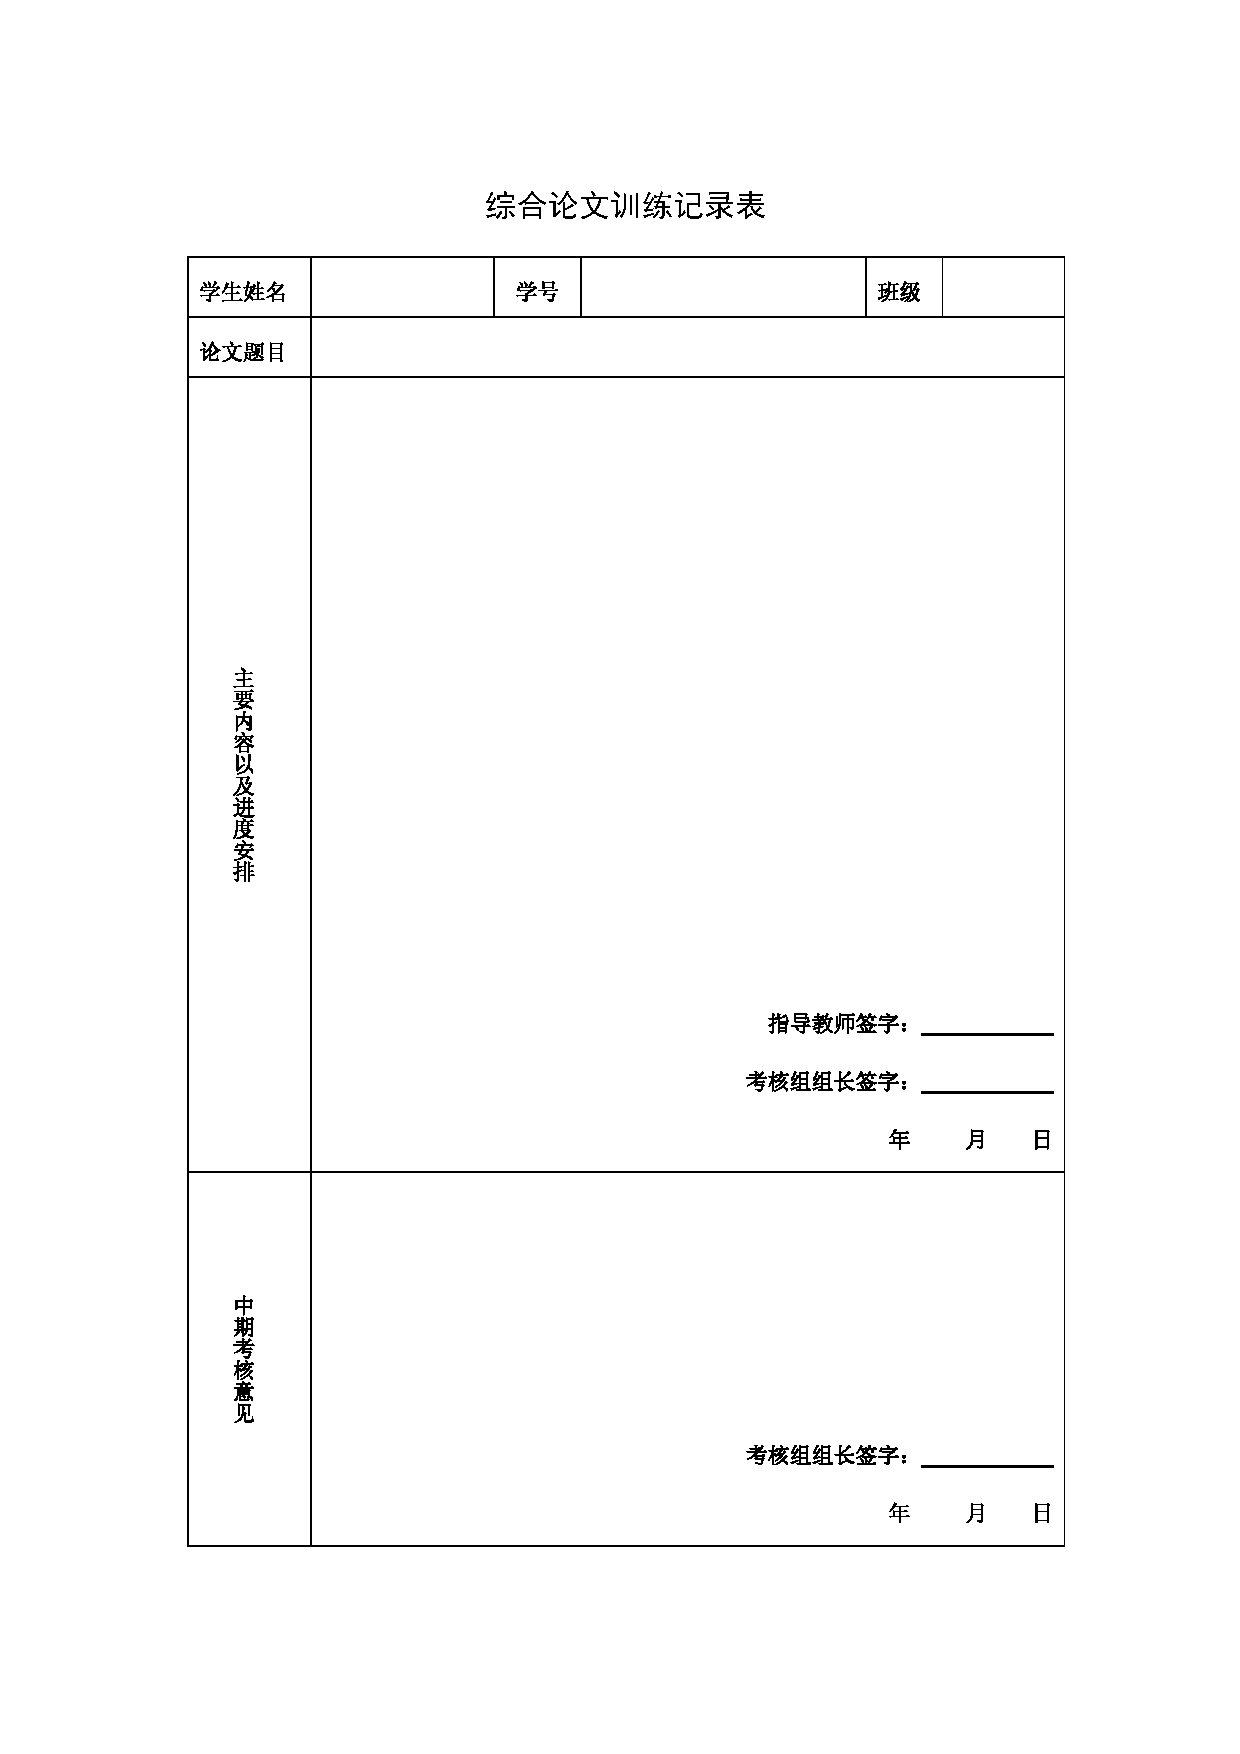
\includepdf[pages=-]{scan-record.pdf}
\end{document}
